

%! TEX root = ../dissertation_gurecky.tex

\section{5x5 Leave-One-Out Machine Learning Results}


Gradient boosted quantile regression model results are presented in figures \ref{fig:qtwallregressionmontagesm} and \ref{fig:qtkeregressionmontagesm}.  For each pin, the predictions are made for the left-out-pin and compared to the original CFD training data.  The gradient boosted results are shown as solid lines and the original CFD-CTF data is shown as broken lines. 

The presented quantile regression results are shown as a function of axial position along the rod for the residual surface temperature and TKE distributions, e.g $\hat q_{\tau}(z) = \mathbf b(z) + \varepsilon(z)$, where $\mathbf b(z) = \mu_{\mathrm{cfd}} - \mu_{\mathrm{ctf}}$.   The results were averaged over the 4 azimuthal CTF faces at each axial level in the CTF grid.   The root-mean-square (RMS) error of select quantiles prediction vs axial location are given in each figure.

Figures \ref{fig:qqtwallmontagesm} to \ref{fig:qqtkepinmontage} show quantile-quantile (Q-Q plots) for each pin in the 5x5 LOO results.  Each Q-Q plot summarizes the overall prediction quality afforded by the quantile regression averaged over the entire pin length.  At each CTF axial grid level, the Kolmogorov–Smirnov (KS) statistic was computed to quantify the goodness-of-fit of the quantile distribution reconstruction to the original, empirical CFD-CTF distribution. The average and maximum KS statistic encountered is recorded in each figure.

Additionally, the predicted rank correlation coefficient as a function of axial position made by the LOO-trained models are compared to the expected result in \ref{fig:ktauregressionmontage}.  The RMS error between the predicted $\hat \rho_\tau(z)$ and the CFD computed $\rho_\tau(z)$ is shown in each figure.

\newgeometry{left=1cm,right=1cm,top=1cm,bottom=1.5cm}
\begin{landscape}
\begin{figure}[H]
    \centering
    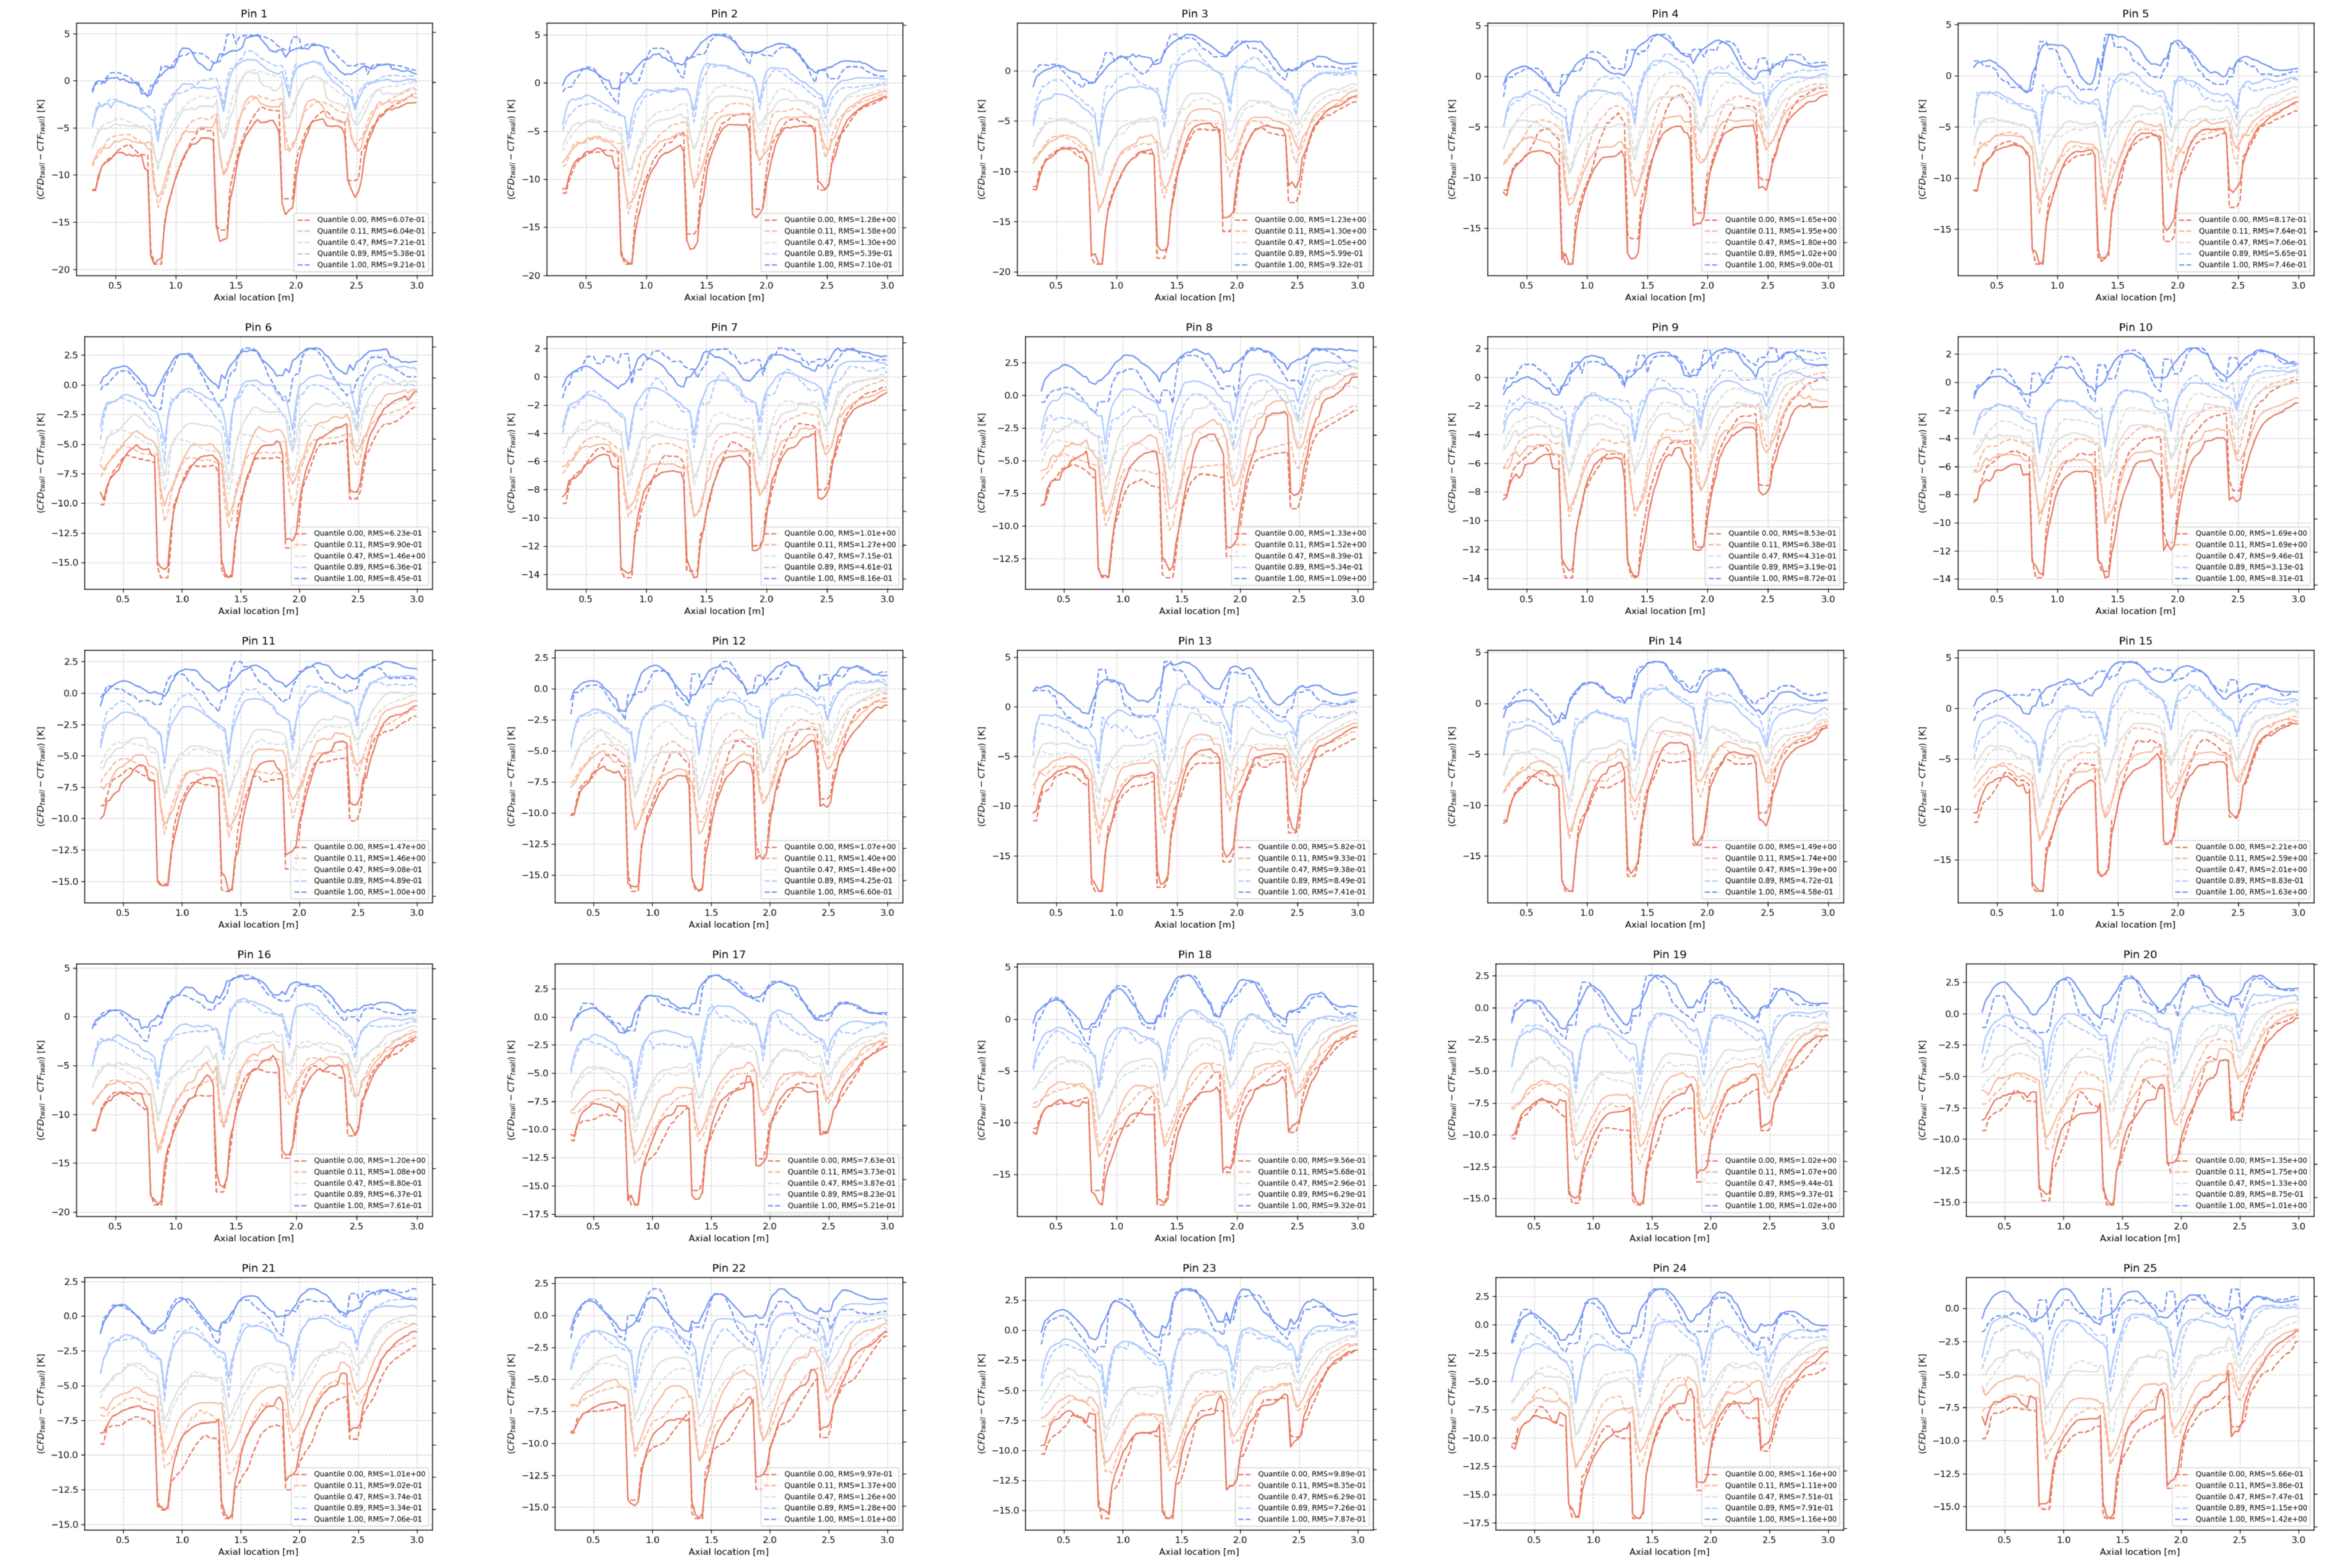
\includegraphics[width=0.96\linewidth]{figs/ml_fit/q_twall_regression_montage_sm}
    \caption{5x5 Axial surface temperature residual (CFD-CTF)  quantile predictions.}
    \label{fig:qtwallregressionmontagesm}
\end{figure}

\begin{figure}[H]
    \centering
    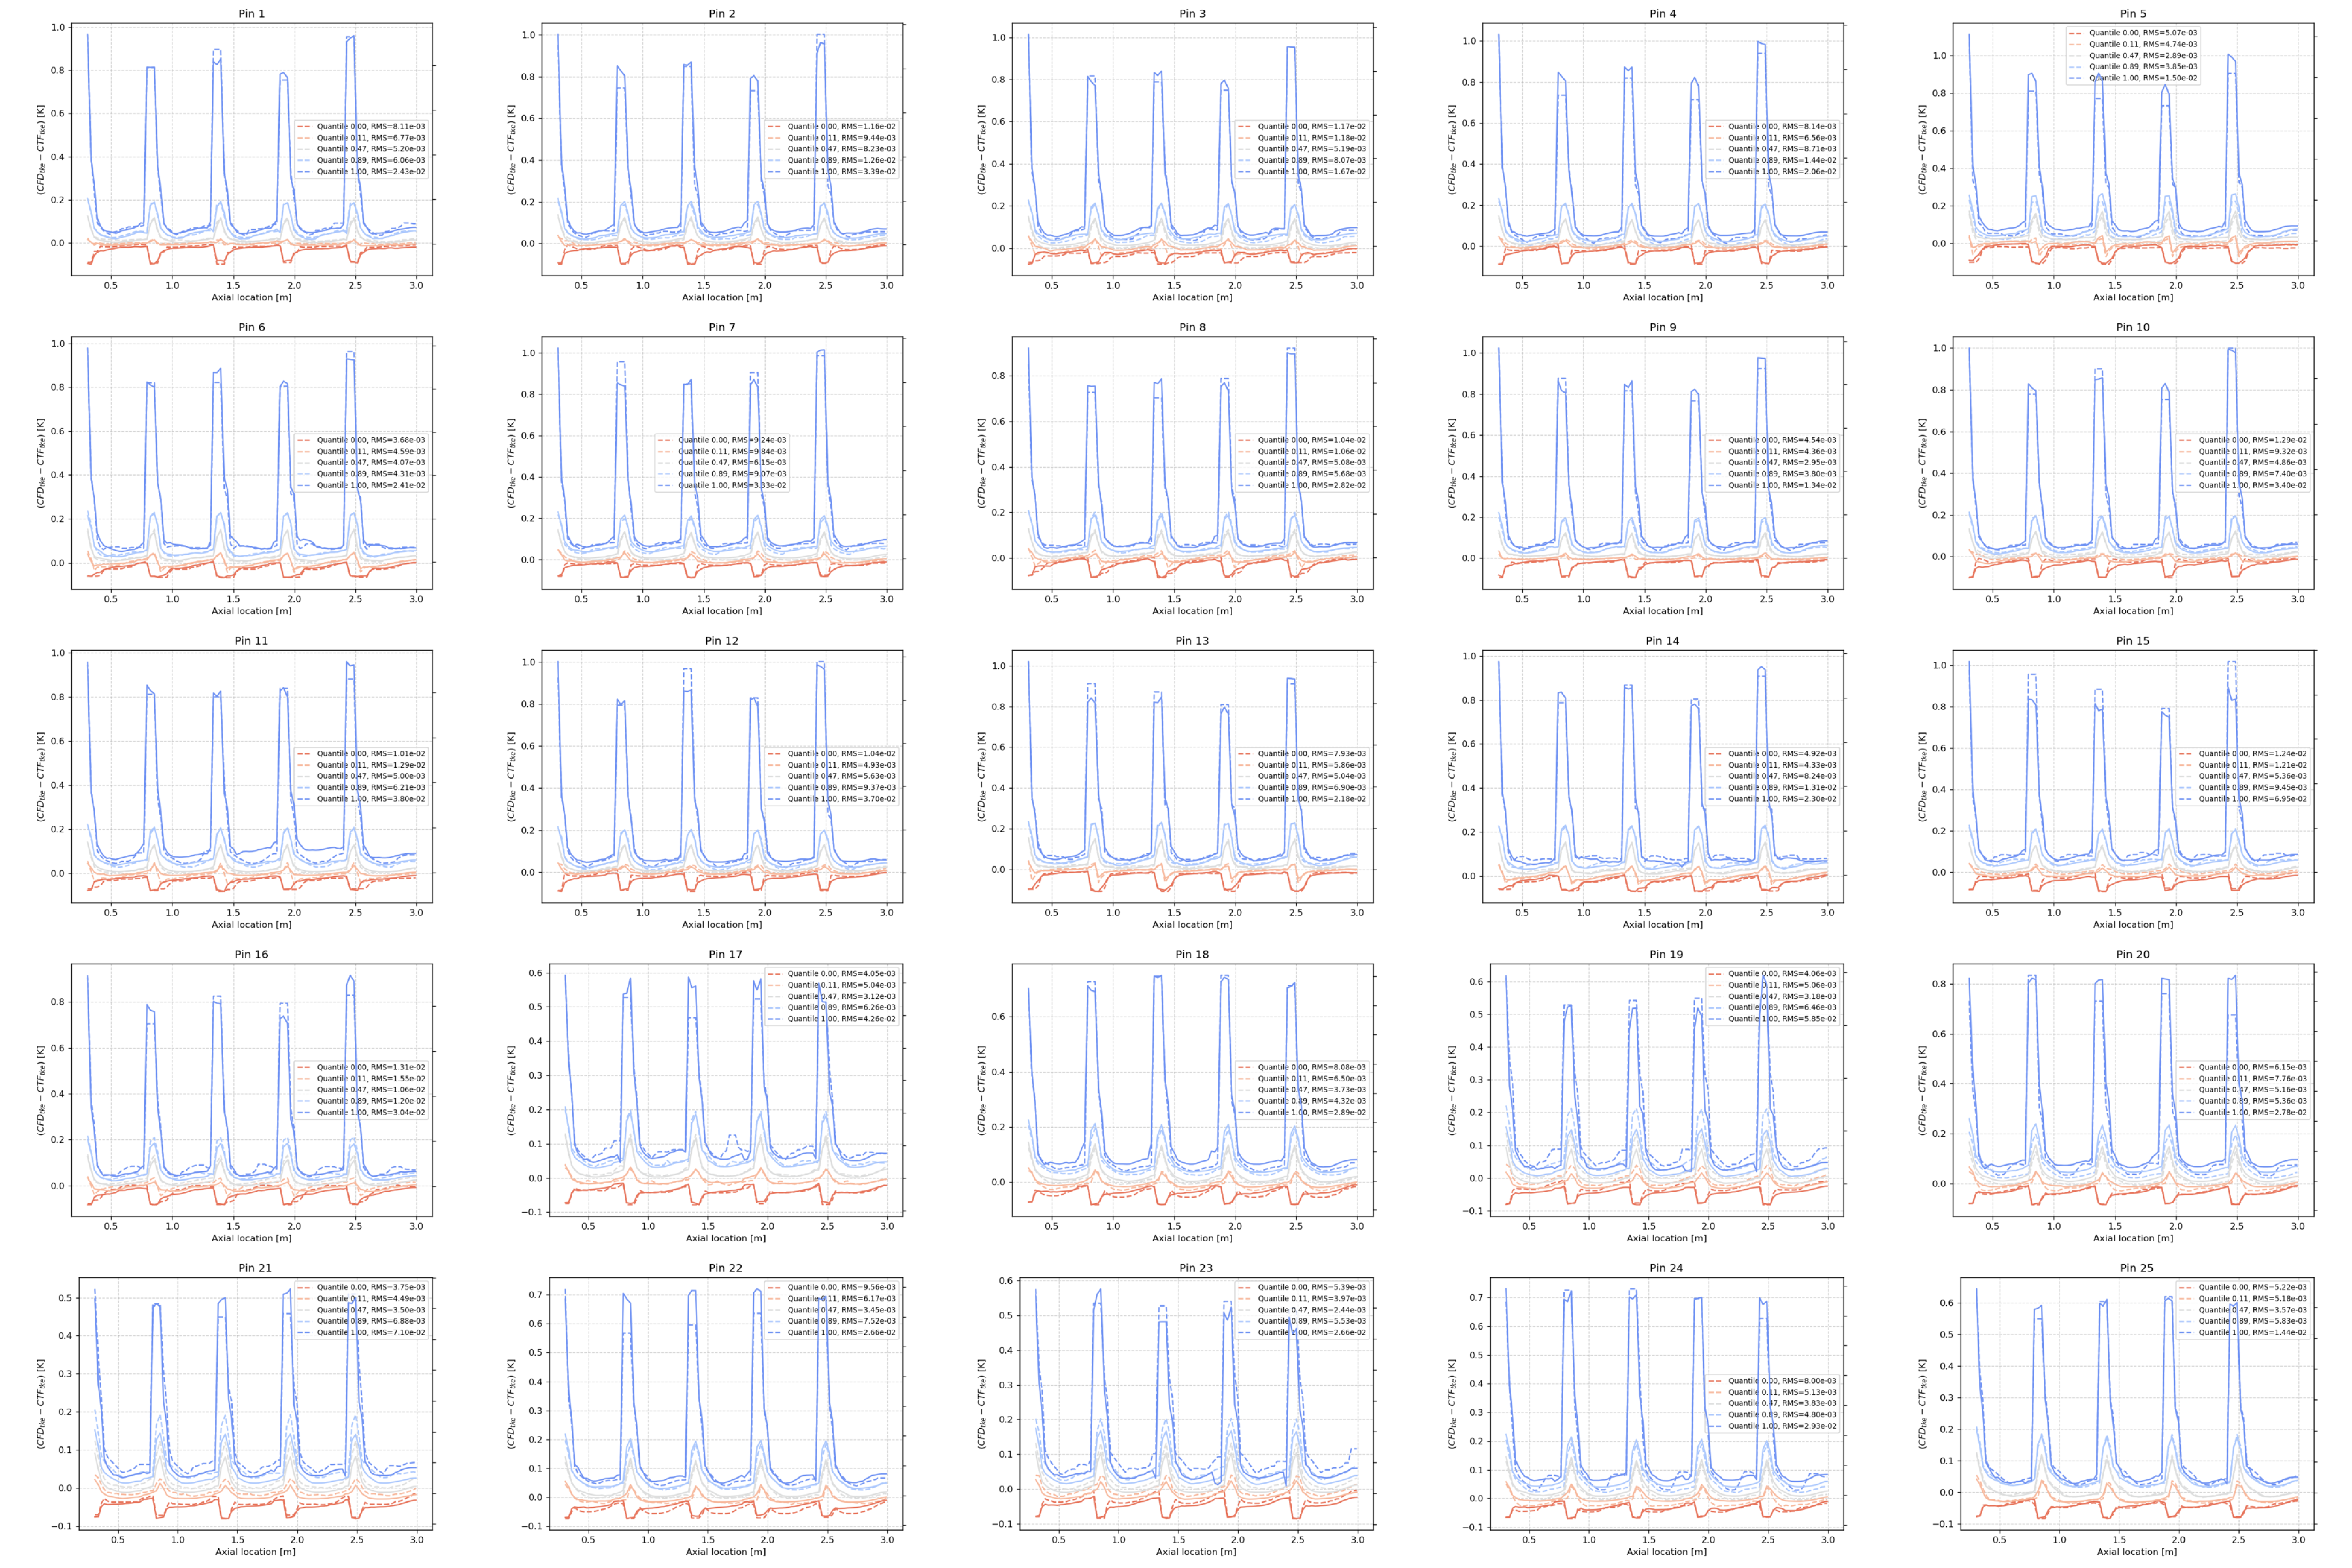
\includegraphics[width=0.96\linewidth]{figs/ml_fit/q_tke_regression_montage_sm}
    \caption{5x5 Axial TKE residual (CFD-CTF) quantile predictions.}
    \label{fig:qtkeregressionmontagesm}
\end{figure}

\begin{figure}[H]
    \centering
    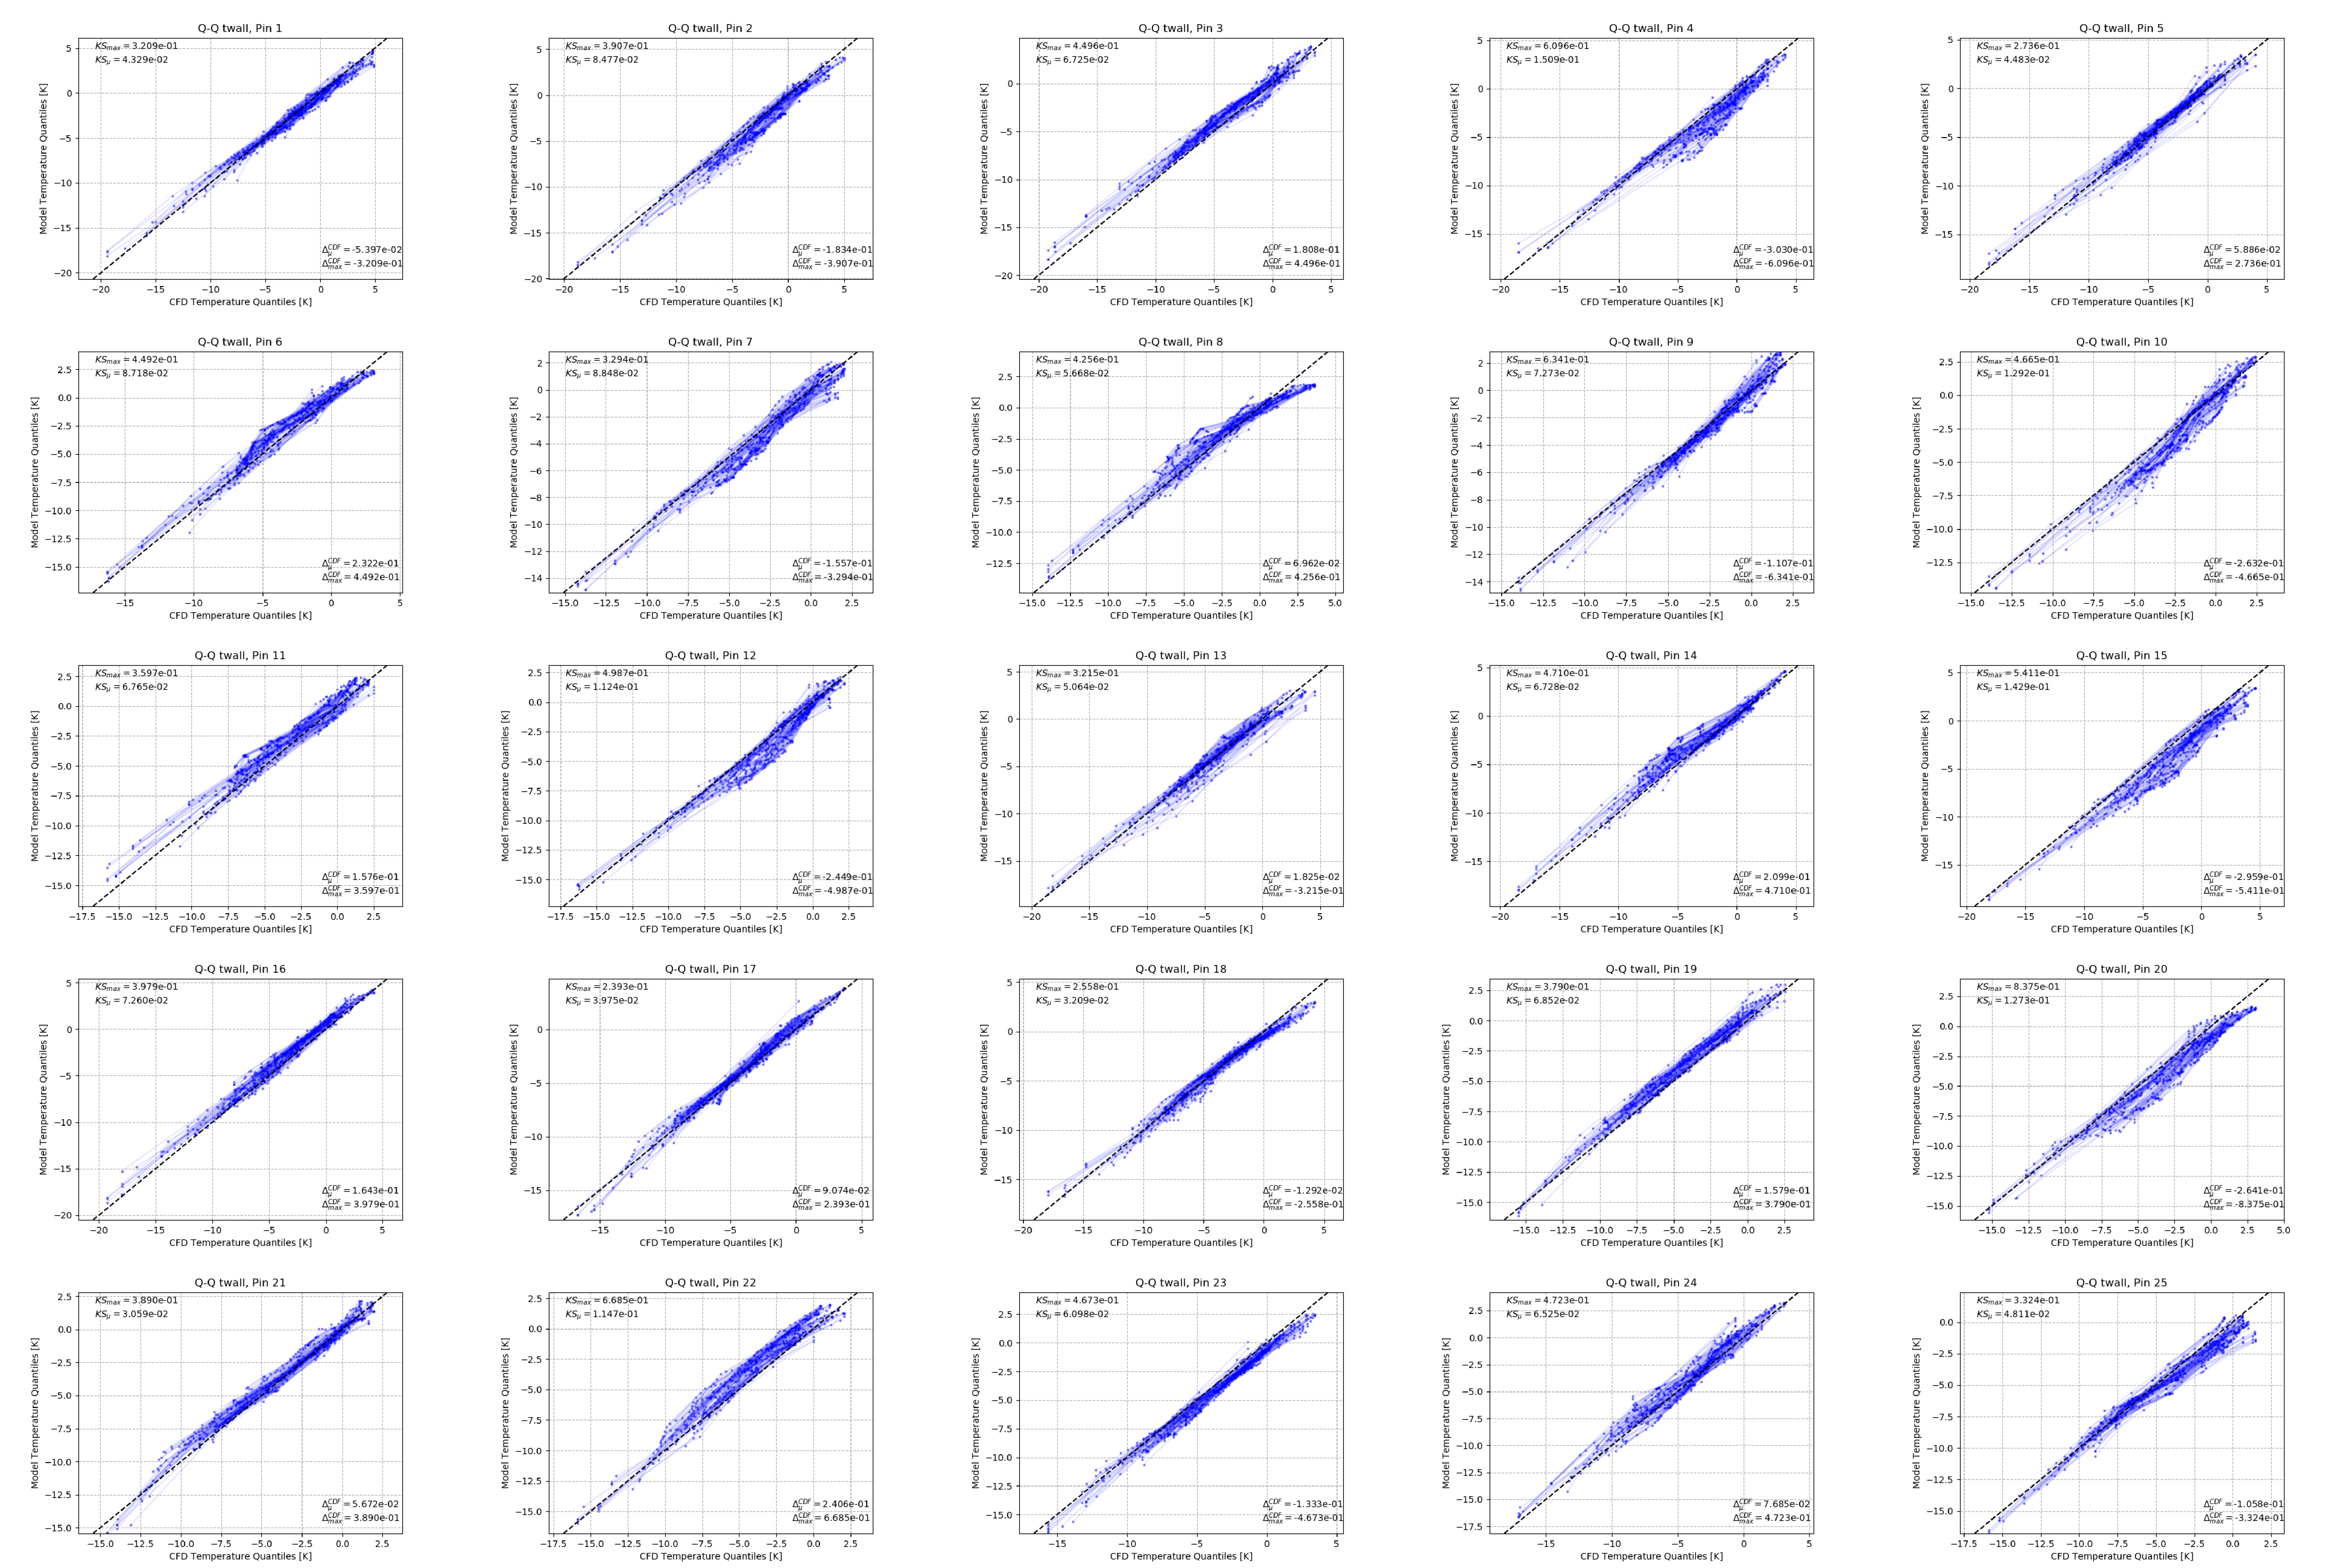
\includegraphics[width=0.96\linewidth]{figs/ml_fit/qq_twall_montage_sm}
    \caption{5x5 surface temperature quantile predictions Q-Q goodness-of-fit summary.}
    \label{fig:qqtwallmontagesm}
\end{figure}

\begin{figure}[H]
    \centering
    \includegraphics[width=0.96\linewidth]{figs/ml_fit/qq_tke_pin_montage}
    \caption{5x5 TKE quantile predictions Q-Q goodness-of-fit summary.}
    \label{fig:qqtkepinmontage}
\end{figure}

\begin{figure}[H]
    \centering
    \includegraphics[width=0.96\linewidth]{figs/ml_fit/ktau_regression_montage}
    \caption{5x5 Kendall's $\tau$ vs axial position predictions.}
    \label{fig:ktauregressionmontage}
\end{figure}
\end{landscape}
\restoregeometry

